\chapter{Open Training Recipes for Reasoning in Language Models}
\label{chap:lec04_open_training_recipes_reasoning}
\section{本讲学习目标}
\begin{itemize}
\item 理解为什么开放生态与可复现 recipe 是 reasoning 研究的前提条件。
\item 分清楚 SFT、preference tuning、RLVR 与 test-time scaling 的职责边界。
\item 看懂 DPO 与 PPO 的关系，以及为什么 data quality 往往比算法标签更重要。
\item 理解 s1 / s1K / budget forcing 如何把训练阶段与测试时推理衔接起来。
\end{itemize}

\section{背景与问题设置}
\subsection{为什么本讲先讲 open recipe，而不是直接讲一个 reasoning 技巧}
Hanna Hajishirzi 一开始就把话题放在 open ecosystem 上，这不是铺垫，而是 lecture 的方法论中心。她的核心论点是：当训练数据、权重、配方、评估和工具链无法被研究者检查时，很多所谓的 “best practices” 其实无法真正变成科学知识。对 reasoning model 尤其如此，因为我们讨论的不是单一 prompt trick，而是一条跨越预训练、后训练和测试时计算分配的工艺链。

\begin{figure}[H]
\centering
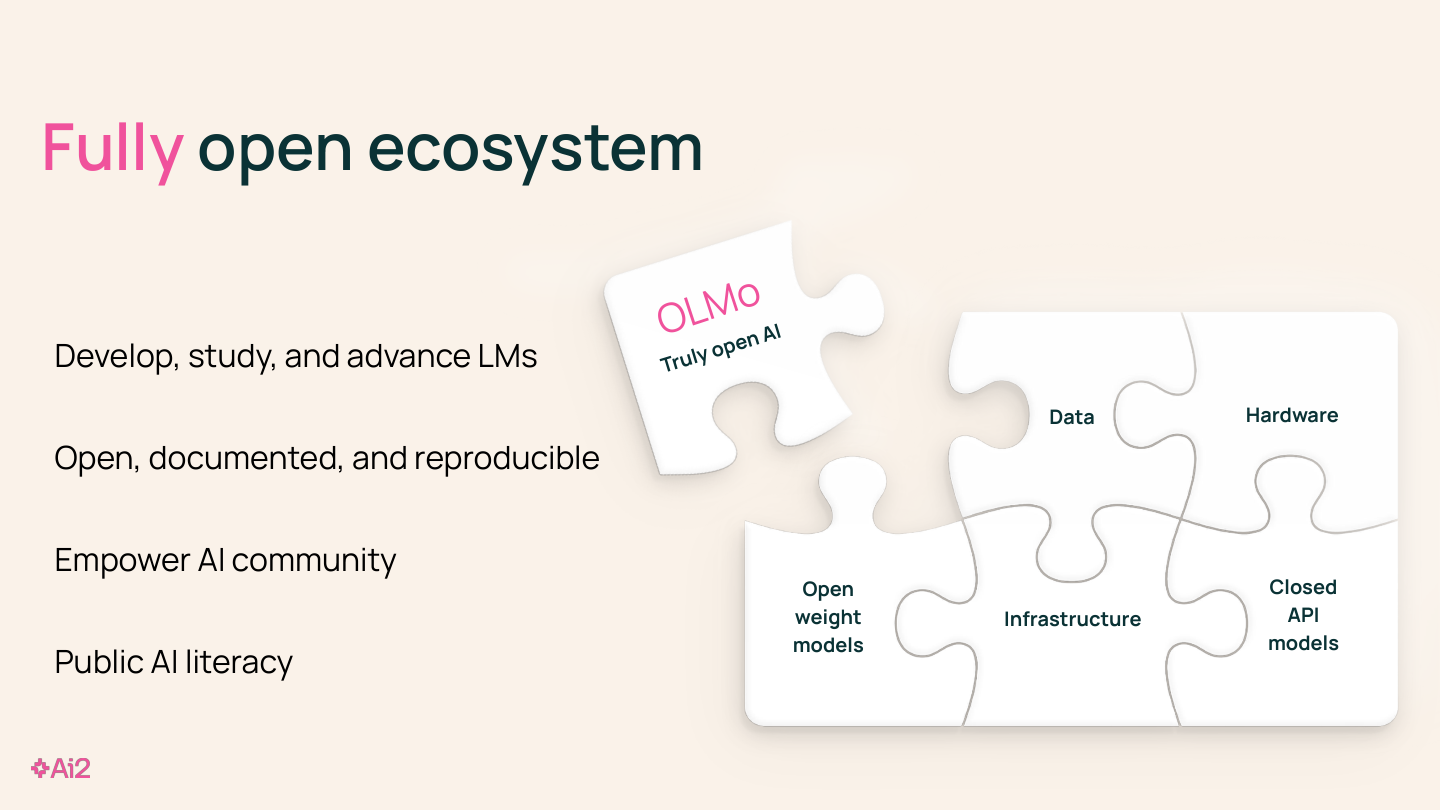
\includegraphics[width=0.82\textwidth]{../lectures/lec04_open_training_recipes_reasoning/figures/lec04_fig_001.png}
\caption{开放语言模型生态图：开放数据、开放工具、开放权重与开放基础设施一起决定 recipe 能否被复做。}
\end{figure}

Slides 对 fully open 的要求也讲得非常明确：不仅要开放模型权重，还要尽可能让训练过程透明、让他人可以访问、复现并质疑数据与配方。这个要求和 agent 课程的关系非常直接：如果你想比较不同 reasoning recipe 的效果，没有可复现的 evaluator 和配方，你根本无法知道性能变化来自哪里。

\begin{figure}[H]
\centering
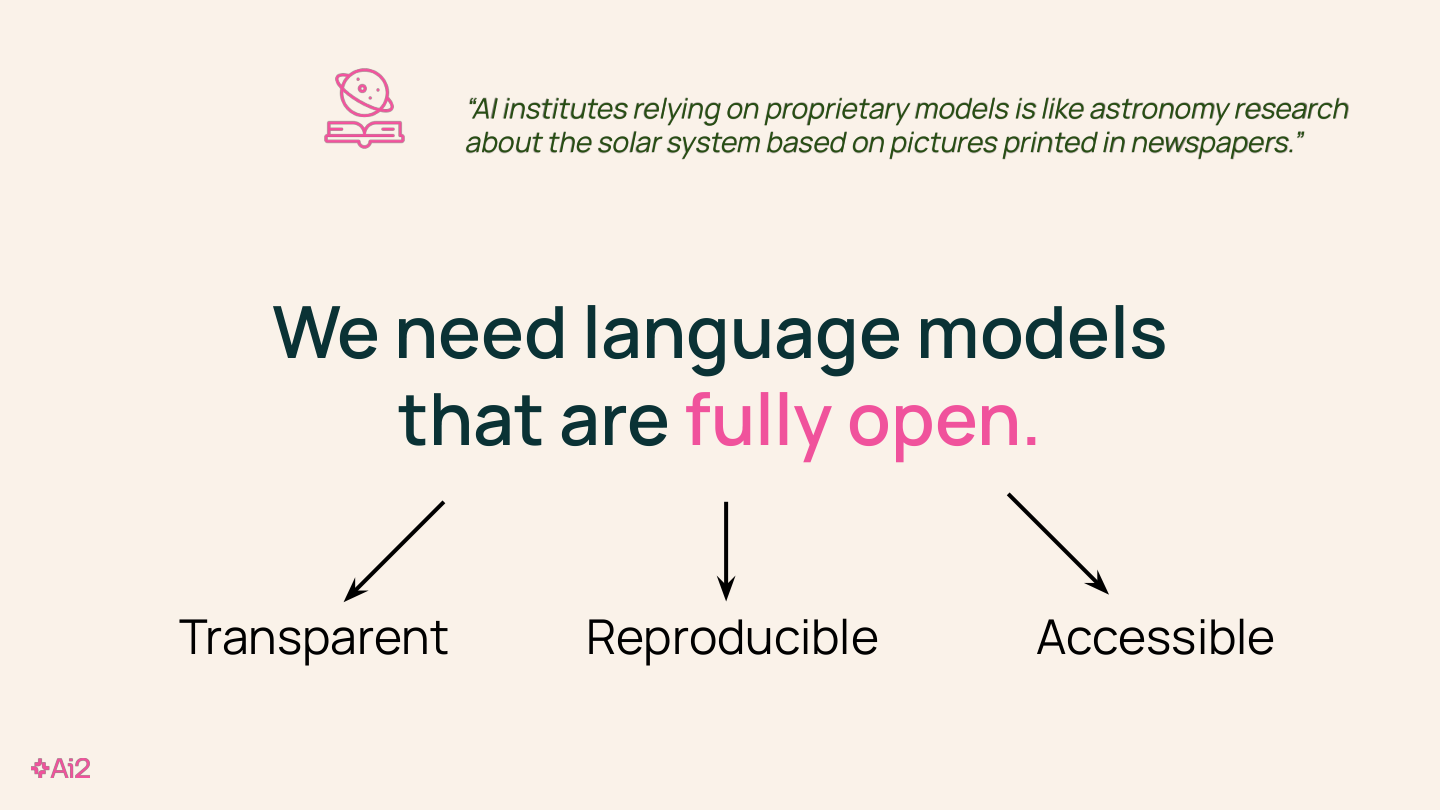
\includegraphics[width=0.76\textwidth]{../lectures/lec04_open_training_recipes_reasoning/figures/lec04_fig_002.png}
\caption{本讲对 fully open 的要求：transparent、reproducible、accessible。}
\end{figure}

\begin{knowledgebox}{本讲的统一视角}
本讲把 reasoning 训练看成一条 staged recipe：先准备 base model，再用不同监督信号逐层塑形，最后在 inference time 把额外预算投到最值得扩展的推理步骤上。
\end{knowledgebox}

\subsection{预训练、后训练与测试时推理的三段式视角}
Slides 第 9--10 页把整个问题拆成三个阶段：pre-training、post-training、test-time inference。这个拆法看似简单，但它避免了一个常见误区：把 reasoning 只当成部署时的 prompt engineering。Hajishirzi 的意思是，想要稳定的 reasoning 行为，训练与测试时必须协同设计。

\begin{figure}[H]
\centering
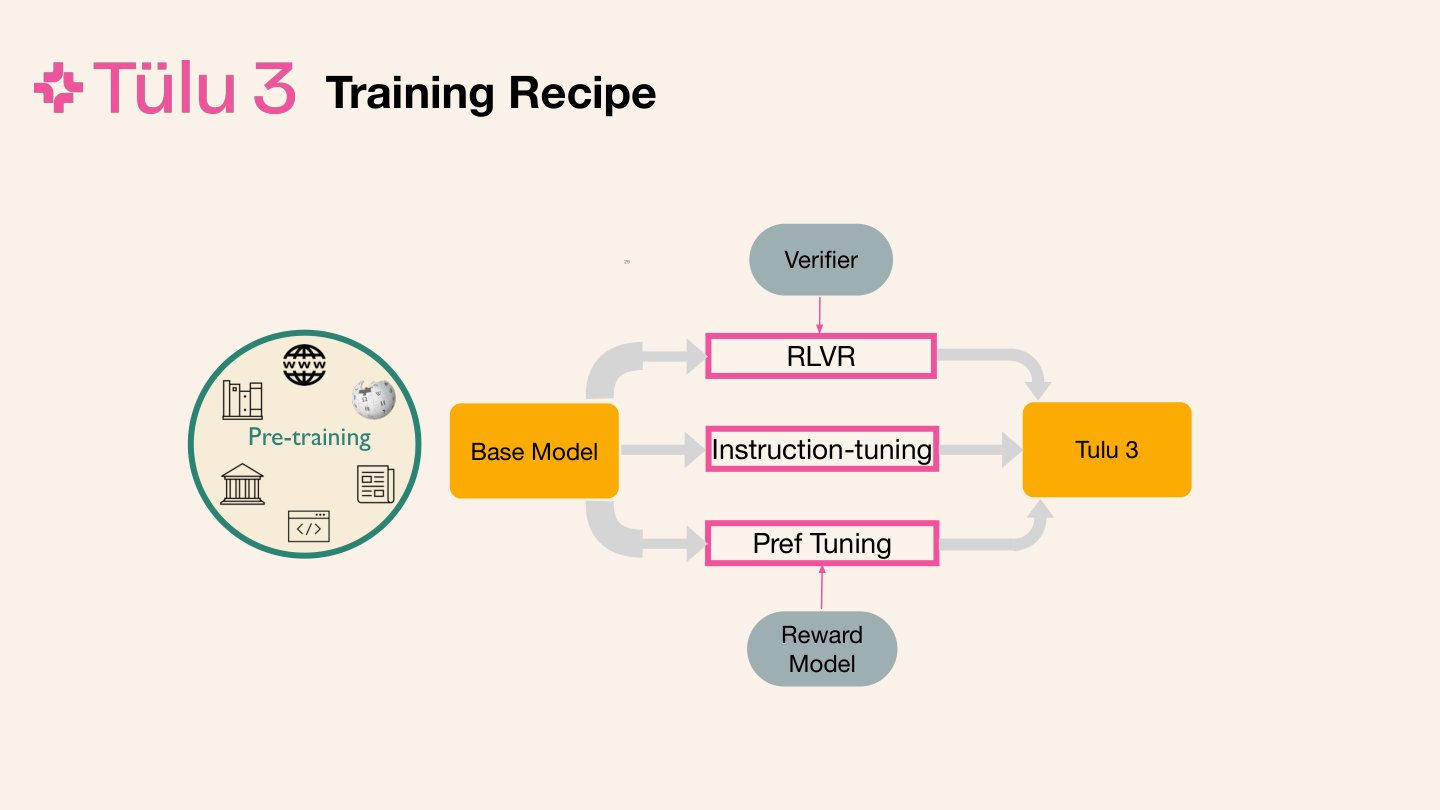
\includegraphics[width=0.83\textwidth]{../lectures/lec04_open_training_recipes_reasoning/figures/lec04_fig_003.png}
\caption{Tulu 3 的阶段化 recipe：base model 之后，按 instruction tuning、preference tuning、RLVR 等阶段逐步增强能力。}
\end{figure}

在这套视角中，监督微调负责把模型从“会续写”变成“会按任务格式做事”；preference tuning 负责把输出风格和偏好对齐；RLVR 负责在存在可验证答案的任务上进一步放大 reasoning 正确率；test-time scaling 则负责在部署时继续把预算换成更高质量的推理轨迹。

\[
\mathcal{L}_{\mathrm{SFT}}(\theta) = -\sum_{(x,y) \in \mathcal{D}_{\mathrm{inst}}} \sum_{t=1}^{|y|} \log p_{\theta}(y_t \mid x, y_{<t})
\]

上式是 lecture 中 supervised finetuning 的数学化抽象。Slides 虽然没有写出完整公式，但它讲的本质就是：给定 instruction-response 配对数据，最大化目标回答的条件概率。这里每个符号的含义分别是：$\mathcal{D}_{\mathrm{inst}}$ 表示 instruction 数据集，$x$ 是 prompt，$y$ 是期望输出，$p_{\theta}$ 是当前策略模型。

\section{监督微调与数据 recipe}
\subsection{SFT 的难点不是目标函数，而是数据从哪里来}
Lecture 对 SFT 的讲法很克制。Hajishirzi 没有把重点放在损失函数，而是强调 data curation, data mixing 和 quality control。因为 instruction tuning 最大的难点不是优化器，而是你到底拿什么数据把模型往哪个能力方向推。

\begin{figure}[H]
\centering
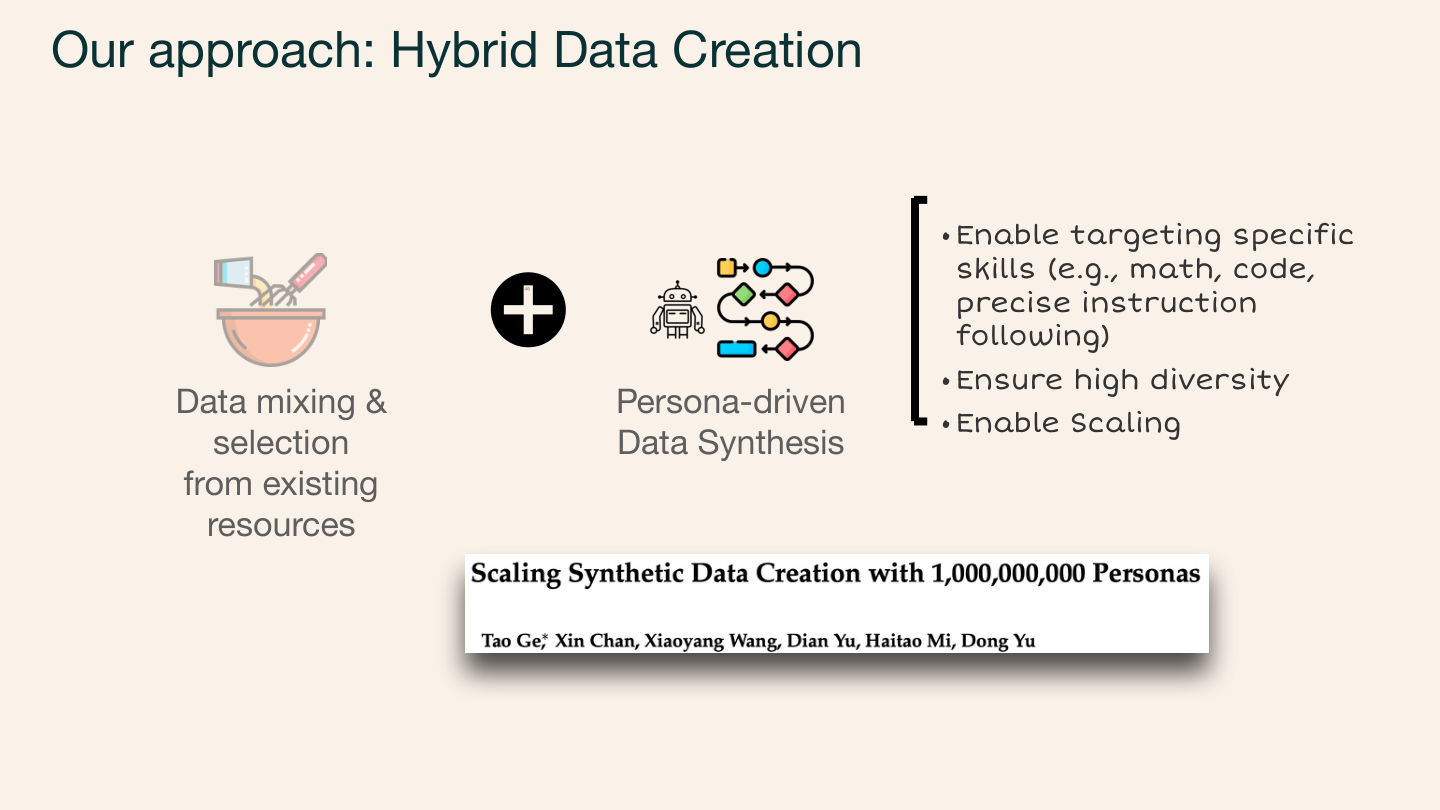
\includegraphics[width=0.82\textwidth]{../lectures/lec04_open_training_recipes_reasoning/figures/lec04_fig_004.png}
\caption{Persona-driven data creation：通过 persona 与目标能力来控制 synthetic reasoning/coding/instruction-following 数据。}
\end{figure}

Slides 连续展示了 Self-Instruct、公开 instruction datasets、hybrid preferences、persona-driven data synthesis 等材料。它们的共同点是：都在尝试用更便宜、更可扩展的方式补齐昂贵的人类标注。尤其是 persona-driven synthesis，它的价值不在于 “合成数据越多越好”，而在于你可以按 math、coding、precise instruction following 等目标能力来有控制地生成数据。

\begin{figure}[H]
\centering
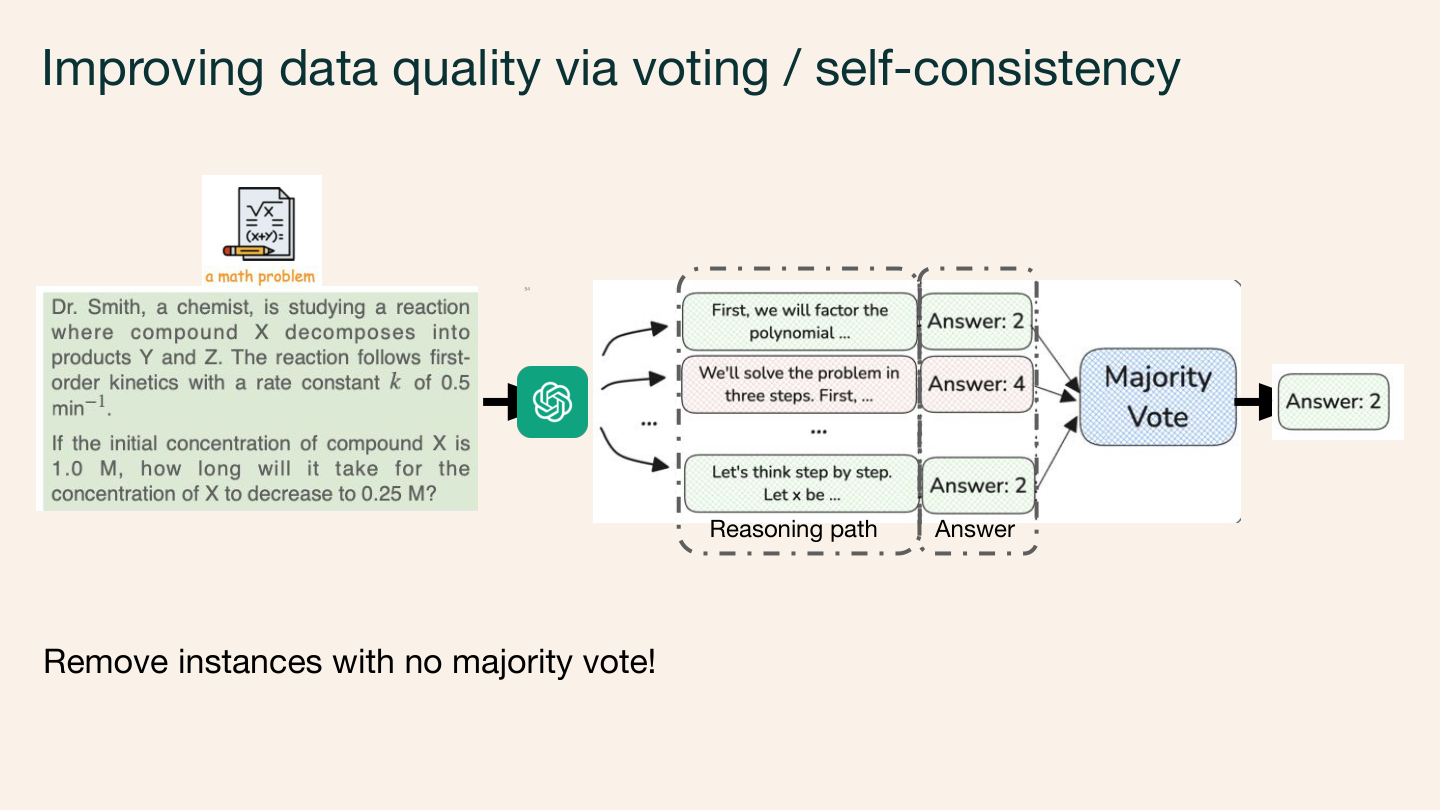
\includegraphics[width=0.75\textwidth]{../lectures/lec04_open_training_recipes_reasoning/figures/lec04_fig_005.png}
\caption{Voting / self-consistency 过滤 reasoning 数据：先用便宜的自动信号筛掉明显不可靠的 traces。}
\end{figure}

这里有一个非常实用的 recipe 观点：reasoning 数据不只是 final answer，更重要的是 reasoning trace 本身。Chain-of-thought 数据有三重作用。第一，它让模型学习多步问题的展开方式；第二，它把错误暴露在中间步骤上；第三，它使数据筛选成为可能，例如通过 voting / self-consistency 保留较可信的样本。

\begin{lstlisting}
capabilities = ['chat', 'knowledge', 'reasoning', 'coding', 'safety']
for cap in capabilities:
    pool = curate_sources(cap)
    filtered = filter_low_quality(pool)
    mixture.extend(sample_with_budget(filtered, target=cap))
\end{lstlisting}

这段伪代码体现的是 lecture 的真正工程逻辑：先定义能力类别，再分别收集、过滤、采样，而不是把一切数据丢进一个大桶里训练。

\begin{importantbox}{为什么朴素地“多收一点数据”不够}
Slides 反复强调许可证检查、去污染（decontamination）、目标能力驱动的 evaluator，以及 mixture balancing。没有这些步骤，更多数据很可能只是更多噪声，甚至会让 reasoning 能力和安全能力互相干扰。
\end{importantbox}

\subsection{Tulu 3 reading 如何补全 lecture 中的 recipe 细节}
《Tulu 3》把 lecture 中的经验写成了论文级 recipe。它最有价值的地方不是某个单一技术点，而是清楚展示了 open post-training 需要哪些材料同时开源：数据、代码、训练脚本、评测、模型以及中间设计权衡。lecture 本身更多讲“怎么想”，而 reading 给出了“怎么复做”。

\section{Preference tuning：DPO 与 PPO 的边界}
Slides 在第 66--78 页把 RLHF 结构拆得非常清楚：prompt 进入 policy，得到多个 response；人类或 AI feedback 形成 preference data；然后你可以训练 reward model，再做 PPO，或者走 DPO 这条更直接的路。

\begin{figure}[H]
\centering
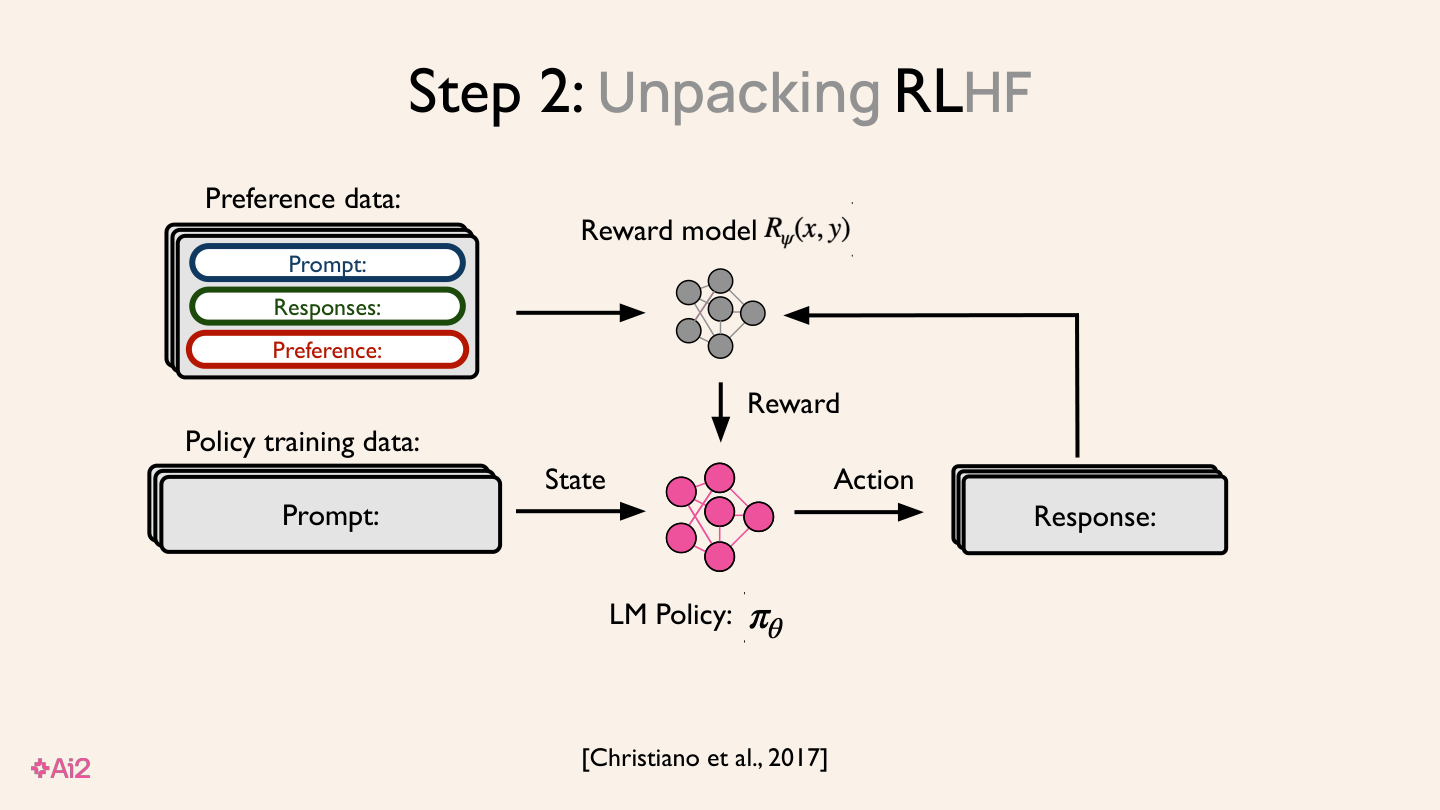
\includegraphics[width=0.84\textwidth]{../lectures/lec04_open_training_recipes_reasoning/figures/lec04_fig_006.png}
\caption{RLHF 组件分解图：preference learning 本质上是在 prompts、responses、reward model 与 policy optimization 之间组织监督信号。}
\end{figure}

\[
\max_{\pi_\theta} \ \mathbb{E}_{x, y \sim \pi_\theta}[r_\phi(x,y)] - \beta \operatorname{KL}(\pi_\theta(\cdot \mid x) \| \pi_{\mathrm{ref}}(\cdot \mid x))
\]

这个 KL-regularized objective 对应 lecture 中 “不要离 base model 太远” 的直觉。$r_{\phi}$ 是 reward model，$\pi_{\theta}$ 是当前 policy，$\pi_{\mathrm{ref}}$ 是 reference model，$\beta$ 控制偏离 reference model 的代价。

\[
\mathcal{L}_{\mathrm{DPO}}(\theta) = -\log \sigma\left(\beta \left[\log \frac{\pi_\theta(y^+\mid x)}{\pi_{\mathrm{ref}}(y^+\mid x)} - \log \frac{\pi_\theta(y^-\mid x)}{\pi_{\mathrm{ref}}(y^-\mid x)}\right]\right)
\]

DPO 的关键在于：不用显式训练 reward model 也能直接利用 preference pairs。这里 $y^+$ 与 $y^-$ 分别表示偏好较好与较差的回答。DPO 的吸引力是实现简单、吞吐高、很适合快速实验；但 lecture 也明确给出工程判断：PPO 通常还能再涨一点，只是更贵、更复杂。

\begin{figure}[H]
\centering
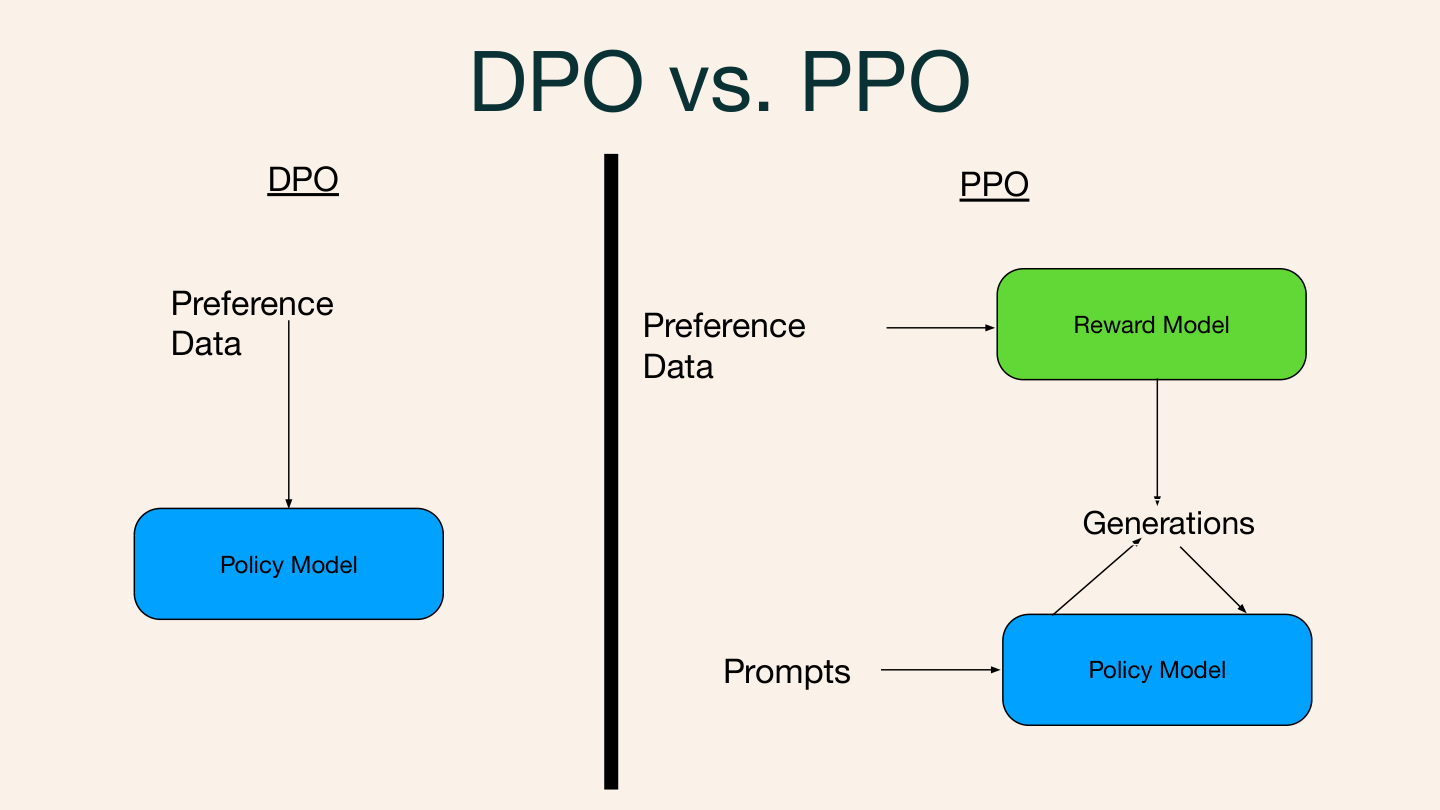
\includegraphics[width=0.78\textwidth]{../lectures/lec04_open_training_recipes_reasoning/figures/lec04_fig_007.png}
\caption{DPO 与 PPO 的训练路径对比。lecture 的重点不是站队，而是理解哪个环节在当前 recipe 中最可能成为瓶颈。}
\end{figure}

\begin{lstlisting}
pairs = collect_preferences(prompts, responses)
if algorithm == 'DPO':
    train_policy_on_pairs(pairs, ref_model)
else:
    reward_model = fit_reward_model(pairs)
    ppo_train(policy, reward_model, prompts)
\end{lstlisting}

《Unpacking DPO and PPO》对这部分的补充很关键。它告诉我们：better preference data 往往比算法标签更重要；更大的 reward model 也不一定自动带来更好的 downstream assistant；policy-training prompts 也有实际影响。换句话说，preference tuning 是系统工程，不是名词工程。

\section{RLVR：在可验证任务上把 reasoning 训练成 RL 问题}
Lecture 在第 97--118 页转向 reinforcement learning with verifiable rewards。这里的关键条件是：任务必须存在可以自动检验的最终答案或约束，例如数学题、可核验 instruction following 或其他 rule-based correctness criterion。

\begin{figure}[H]
\centering
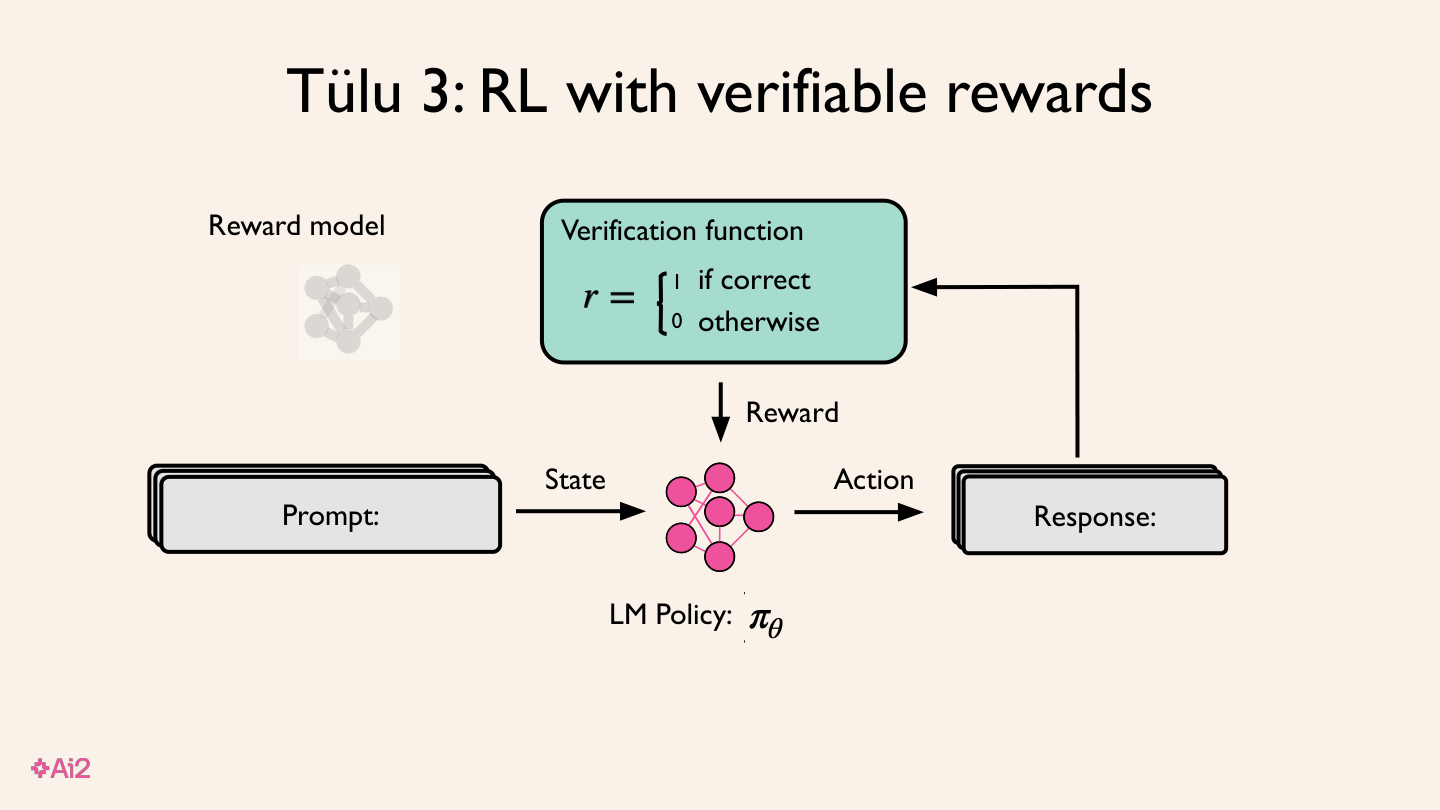
\includegraphics[width=0.8\textwidth]{../lectures/lec04_open_training_recipes_reasoning/figures/lec04_fig_008.png}
\caption{RLVR 的核心结构：不再拟合 reward model，而是直接用 verification function 对最终答案打二值或稀疏奖励。}
\end{figure}

\[
r(x,y) = \mathbf{1}[V(x,y)=1], \qquad \max_{\pi_\theta} \mathbb{E}_{x, y \sim \pi_\theta}[r(x,y)]
\]

这条公式很重要。$V(x,y)$ 是 verification function，检查给定 prompt $x$ 和回答 $y$ 是否满足 gold answer 或规则约束；一旦可验证，奖励 $r(x,y)$ 就可以写成简单的指示函数。这解释了为什么 RLVR 在 reasoning 任务上会突然变得实用：它不需要人类去标每一步 chain-of-thought，只要最终答案可检验即可。

\begin{lstlisting}
for prompt in verifier_dataset:
    answer = policy.sample(prompt)
    reward = verifier(prompt, answer)
    policy = ppo_update(policy, prompt, answer, reward)
\end{lstlisting}

但 lecture 也明确指出了边界：RLVR 更适合 final answer 可验证的任务，不适合开放域聊天；奖励稀疏意味着优化很容易不稳定；而且它未必会学出“优雅”的 reasoning，只会学出“更容易通过 verifier”的策略。因此 verifier 设计、训练集选择和过优化风险非常关键。

\section{s1、budget forcing 与最小 reasoning recipe}
Lecture 最值得和第一讲连起来读的部分，是第 124--142 页关于 s1 的讨论。Hajishirzi 展示了一种令人印象深刻的最小 recipe：只用相对少量但高质量、困难且多样的 reasoning 样本 s1K，再配一个非常简单的 test-time scaling 方法 budget forcing，就可以得到明显的 reasoning 增益。

\begin{figure}[H]
\centering
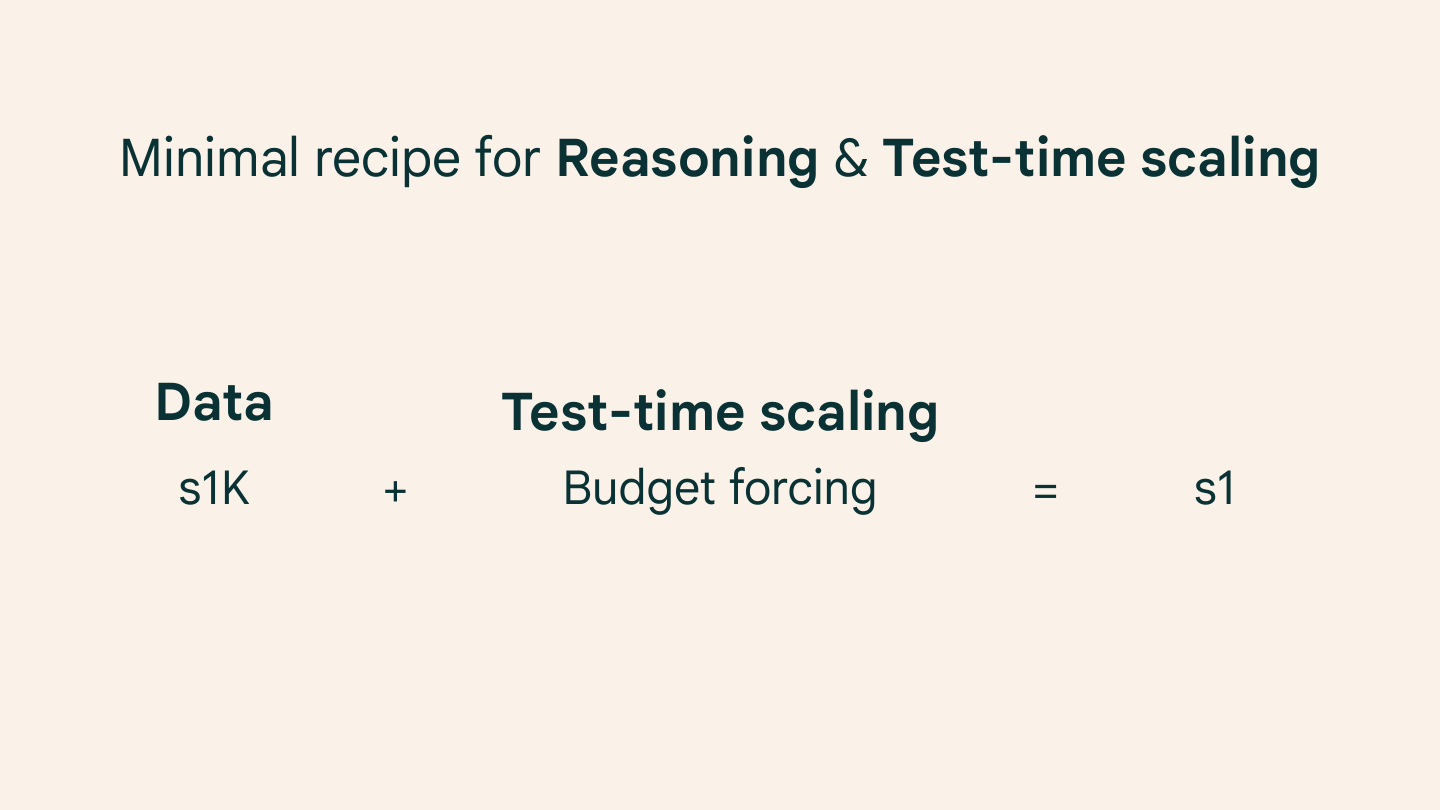
\includegraphics[width=0.79\textwidth]{../lectures/lec04_open_training_recipes_reasoning/figures/lec04_fig_009.png}
\caption{s1 的最小 recipe：高质量 reasoning data 加简单但有效的 budget forcing。}
\end{figure}

\[
y = \operatorname{Decode}(x; B), \qquad B' > B \Rightarrow \text{allow additional reasoning steps or forced continuation tokens}
\]

这个抽象表达的不是某个唯一实现，而是 lecture 的核心思想：你可以显式控制推理预算 $B$，并通过更大的预算 $B'$ 允许更多 reasoning steps，甚至强制继续生成思考过程。Slides 里的 budget forcing 例子之所以重要，在于它说明 reasoning gain 不一定要靠更大模型或更多训练 token，也可以来自更聪明的 test-time compute allocation。

\begin{lstlisting}
answer = policy.generate(prompt, max_tokens=budget)
while not stop(answer) and spent(answer) < forced_budget:
    answer += policy.generate('Wait', continue_from=answer)
\end{lstlisting}

\begin{figure}[H]
\centering
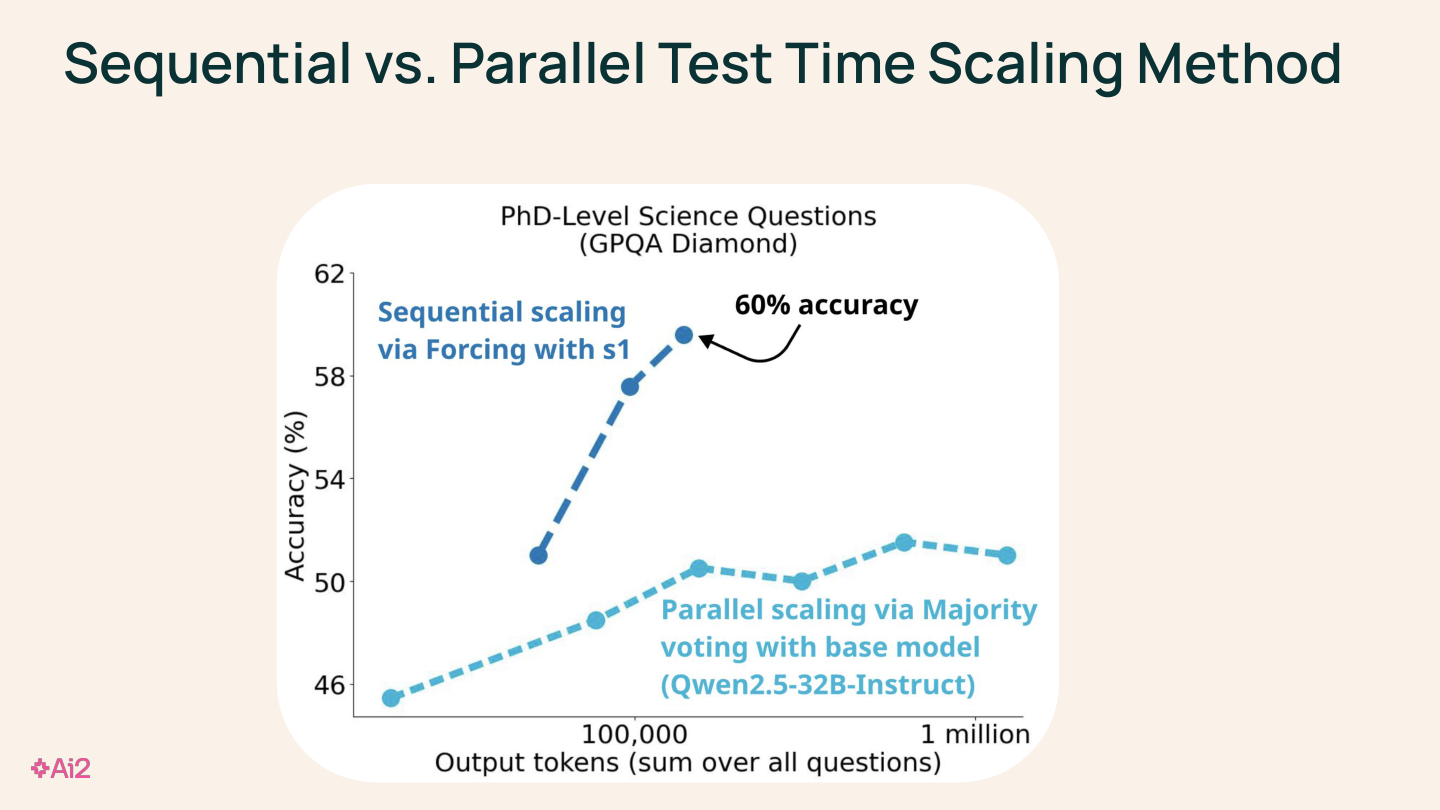
\includegraphics[width=0.82\textwidth]{../lectures/lec04_open_training_recipes_reasoning/figures/lec04_fig_010.png}
\caption{Sequential 与 parallel test-time scaling 的区别：预算可以投在延长单条轨迹，也可以投在扩展候选空间。}
\end{figure}

这一段与第一讲的 inference-time techniques 正好形成闭环：L01 讨论“怎么花 test-time compute”；L04 讨论“训练 recipe 怎样为这种花法做准备”。没有合适的训练数据和 staged post-training，单纯延长思考很可能只会延长错误轨迹。

\section{与关键 readings、前后讲和失败模式的联系}

\subsection{Tulu 3：为什么“开放 recipe”不能只开 checkpoint}

《Tulu 3》是本讲最核心的 reading，因为 lecture 中反复强调的 staged recipe 基本都能在这篇 paper 里找到对应物。它真正说明的是：所谓 open post-training，不是把一个指令模型权重扔出来就结束，而是要把 \textbf{阶段顺序、数据治理、评测方式和复现实践} 一并公开。否则社区只能看到结果，看不到为什么这个结果能成立。

这也解释了 slides 中为何反复出现 data mixture、stage ordering 和 evaluator choice。Tulu 3 的 strongest claim 不是“公开模型也能强”，而是“当 SFT、preference tuning 与 reasoning-oriented RL 被按合适顺序组织时，公开 recipe 可以逼近甚至超过很多强 instruct baseline”。但它同样保留了一个重要限制：\textbf{上游 base model 的能力边界仍然存在}。如果 base model 的长程 reasoning basis 很弱，后面的 recipe 只能局部修正，而很难凭空创造能力。

\subsection{Unpacking DPO and PPO：lecture 的工程判断为什么成立}

《Unpacking DPO and PPO》让本讲对 DPO/PPO 的立场更具体。lecture 并没有说“算法不重要”，而是说\textbf{如果 preference data 和 evaluator 已经不可靠，那么算法名词本身很难救场}。这篇 reading 的系统消融恰好支持这一点：better preference data 往往是最大的杠杆，reward model 规模、policy-training prompt 和学习算法都会影响结果，但它们的作用方式并不等价。

因此 lecture 的工程判断其实有两层。第一层是：PPO 往往还能比 DPO 再涨一点，但代价是更重的实现复杂度、吞吐成本和调参负担。第二层是：对很多开放研究团队而言，\textbf{先把 data quality、prompt construction 和 evaluator 站稳，再比较 DPO/PPO，才是更合理的资源分配顺序}。这也能解释为什么 Hajishirzi 在 slides 里把算法、数据、评测放进同一个 recipe 视角，而不是单独给某个算法封神。

\subsection{OpenScholar：为什么开放基础设施会在下游 agent 中兑现}

《OpenScholar》虽然不是这场 lecture 的主体算法，但它提供了一个非常关键的下游例子：开放模型、开放 retrieval pipeline 和 citation-grounded synthesis 结合后，能够显著降低 citation hallucination。这使它成为 lecture 开头“开放基础设施有技术含义”的直接证据。

更重要的是，它提醒读者：开放 recipe 的价值不止体现在 benchmark leaderboard。真正长期的价值，是它能让 scientific agents、retrieval-augmented assistants 和领域专用系统在 attribution、reproducibility 和 error analysis 上更可控。本讲讲的是 training recipe，而 OpenScholar 展示的是\textbf{这些 recipe 进入下游系统后，会如何改变 agent 的可信度上限}。

本讲最需要警惕的失败模式包括：
\begin{itemize}
\item 把开放误解为只开权重，而忽视数据、配方与评测的可复现性。
\item 把 DPO/PPO 之争当成全部问题，忽视 preference data 与 evaluator 的质量。
\item 在没有可靠 verifier 的任务上生搬硬套 RLVR。
\item 误以为 budget forcing 永远有用，而忽视模型是否已经具备可扩展的 reasoning basis。
\end{itemize}

与前一讲的关系：L01 讲的是 inference-time reasoning methods；本讲解释这些方法为什么需要被训练 recipe 支撑。与下一讲的关系：L05 会把这种 recipe 观念带进 coding agents 和 vulnerability detection，进一步强调 environment feedback 与 verification 的角色。

\section{本章小结}
本讲最重要的教材结论是：reasoning 不是单一阶段的问题，而是贯穿数据、SFT、偏好优化、RL 与 test-time compute allocation 的系统工程。开放 recipe 的价值在于，它让这些决策可以被研究社区真正检验、继承和改进。

\section{复习题}
\begin{itemize}
\item 为什么开放生态在本讲中是技术命题而不只是社区命题？
\item SFT、preference tuning、RLVR 三者在监督信号上有何差别？
\item 为什么 better preference data 往往比 DPO 与 PPO 的标签更重要？
\item RLVR 适用的任务边界是什么？
\item s1 与 budget forcing 如何体现最小 reasoning recipe？
\end{itemize}

\section{深入思考题}
\begin{itemize}
\item 如果你只能做一个阶段改进，你会优先改进 evaluator、data mixture 还是优化算法？为什么？
\item 什么样的 verifier 最容易诱发 reward hacking？如何缓解？
\item 在开放模型研究中，哪些资源最需要被优先开源才能真正支持科学复现？
\end{itemize}

\section{延伸阅读}
\begin{itemize}
\item Tulu 3: Pushing Frontiers in Open Language Model Post-Training
\item Unpacking DPO and PPO: Disentangling Best Practices for Learning from Preference Feedback
\item OpenScholar: Synthesizing Scientific Literature with Retrieval-augmented LMs
\end{itemize}
